To validate the feasibility of the proposed control structure, the individual controllers are tested independently, and the full cascaded structure is then tested in concert. The small-signal model is used for all simulation tests; while this is inherently less accurate than testing against the full nonlinear model \cref{eq:NonLinearModelWithTank}, this model's stiffness requires a sampling interval that, considering the computational complexity of each timestep and the timescale of the dynamics, is impracticable. \textbf{NOTE: Simulation results will be replaced with laboratory results in final draft. No results are presented with respect to the disturbance estimators or packet loss as we are still figuring things out}.

We first present results pertaining to the VF-LQR. The controller is tested against nominal conditions, a variety of non-nominal time constants, and against a constant output disturbance. In each case the controls are clamped corresponding to the provided pump curves \cite{GrundfosDatablad}, the system is subjected to a varying state disturbance, and a sampling time of $t_s = 10\si{min}$ is assumed. The results can be seen on \cref{fig:LQRTracking}, displaying good tracking performance in each case; the disturbance is completely rejected, and the system tracks the reference. In all cases $Q = \left(\tilde{C}^T\tilde{C}\right)$ and $R = \text{diag}(0.1)$; the former guarantees an exponentially stable closed-loop system \cite{Liberzon2012}.


\begin{figure}[h!]
	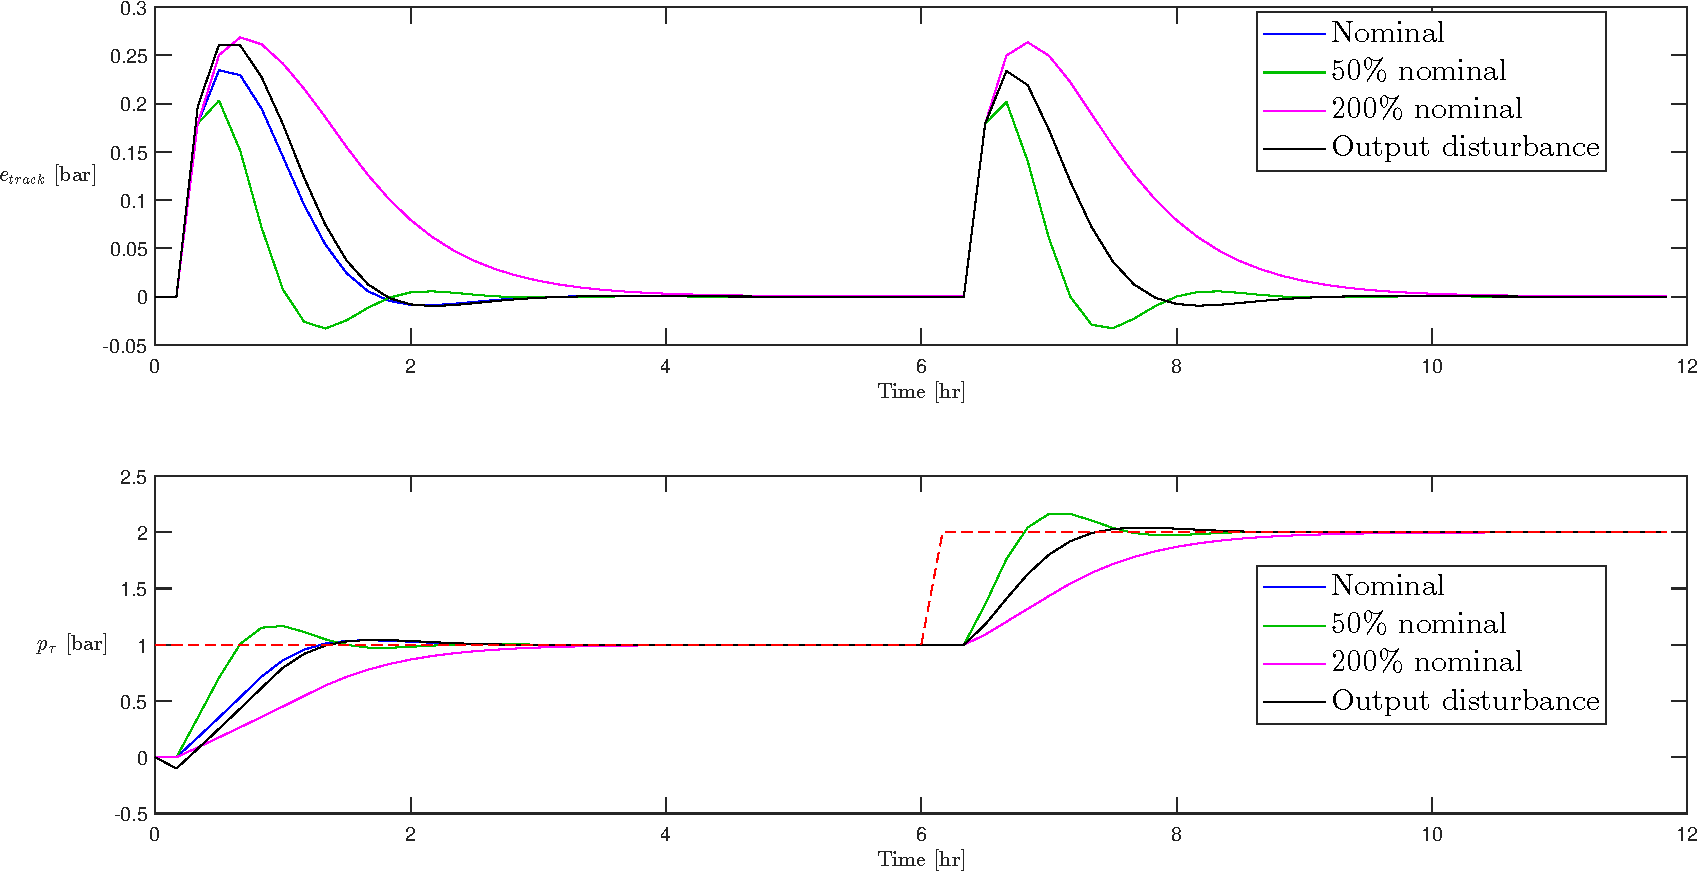
\includegraphics[height=4cm, width=\linewidth]{Graphics/LQRTracking.pdf}
	\caption{Outer loop simulation.}
	\label{fig:LQRTracking}
\end{figure}

 We now examine the behaviour of the inner loop under two separate step references on \cref{fig:PumpSimulation}. The PID controllers are limited to the range $\{-66,34\}$, corresponding to the inputs $\{0,100\}$ to the full system, with a back-calculation anti-windup scheme.

\begin{figure}[h!]
	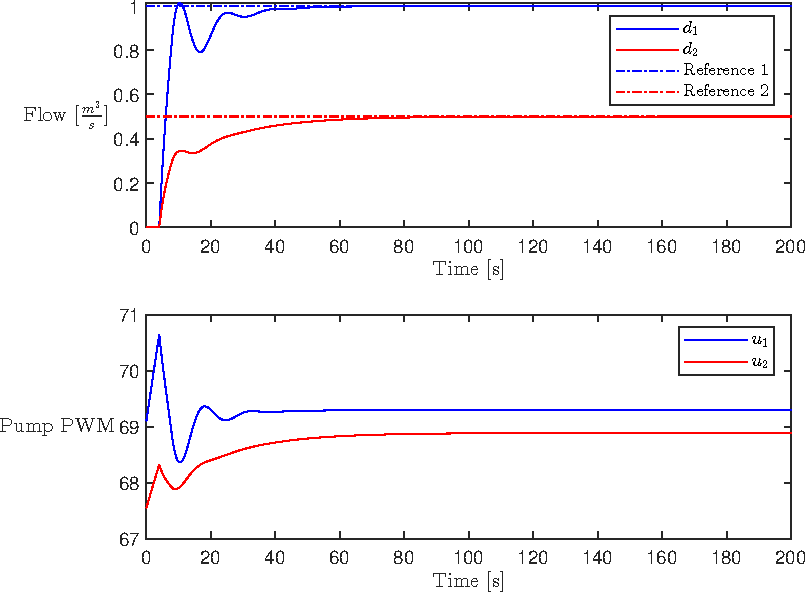
\includegraphics[width=\linewidth,height=4cm]{Graphics/PumpSimulation.pdf}
	\caption{Inner loop simulation.}
	\label{fig:PumpSimulation}
\end{figure}

The results on \cref{fig:PumpSimulation} show a convergence speed of roughly $40 \si{s}$ and limited ringing as desired. Finally, we evaluate the full cascaded control structure, again under the influence of a time-varying disturbance.

\begin{figure}[h!]
	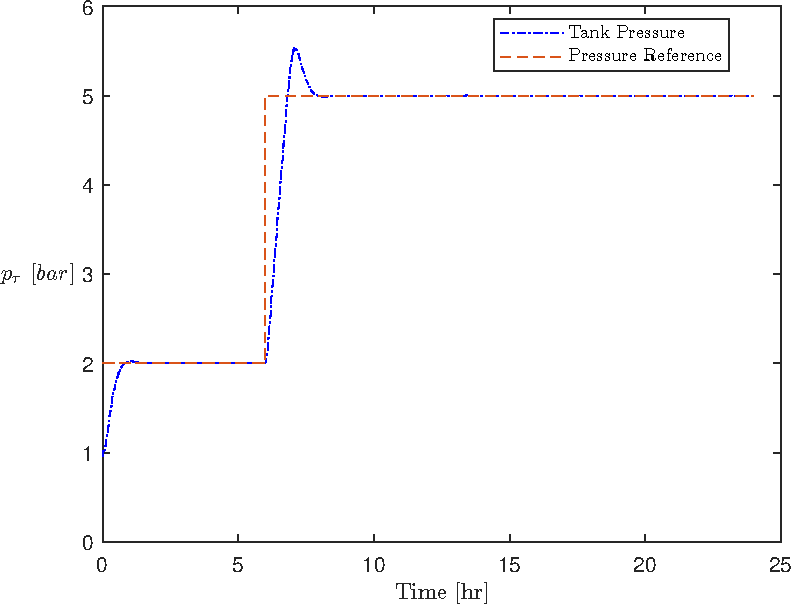
\includegraphics[height=4cm, width=\linewidth]{Graphics/FullSimPressures.pdf}
	\caption{Outer loop, cascaded simulation.}
	\label{fig:FullSimPressure}
\end{figure}

\begin{figure}[h!]
	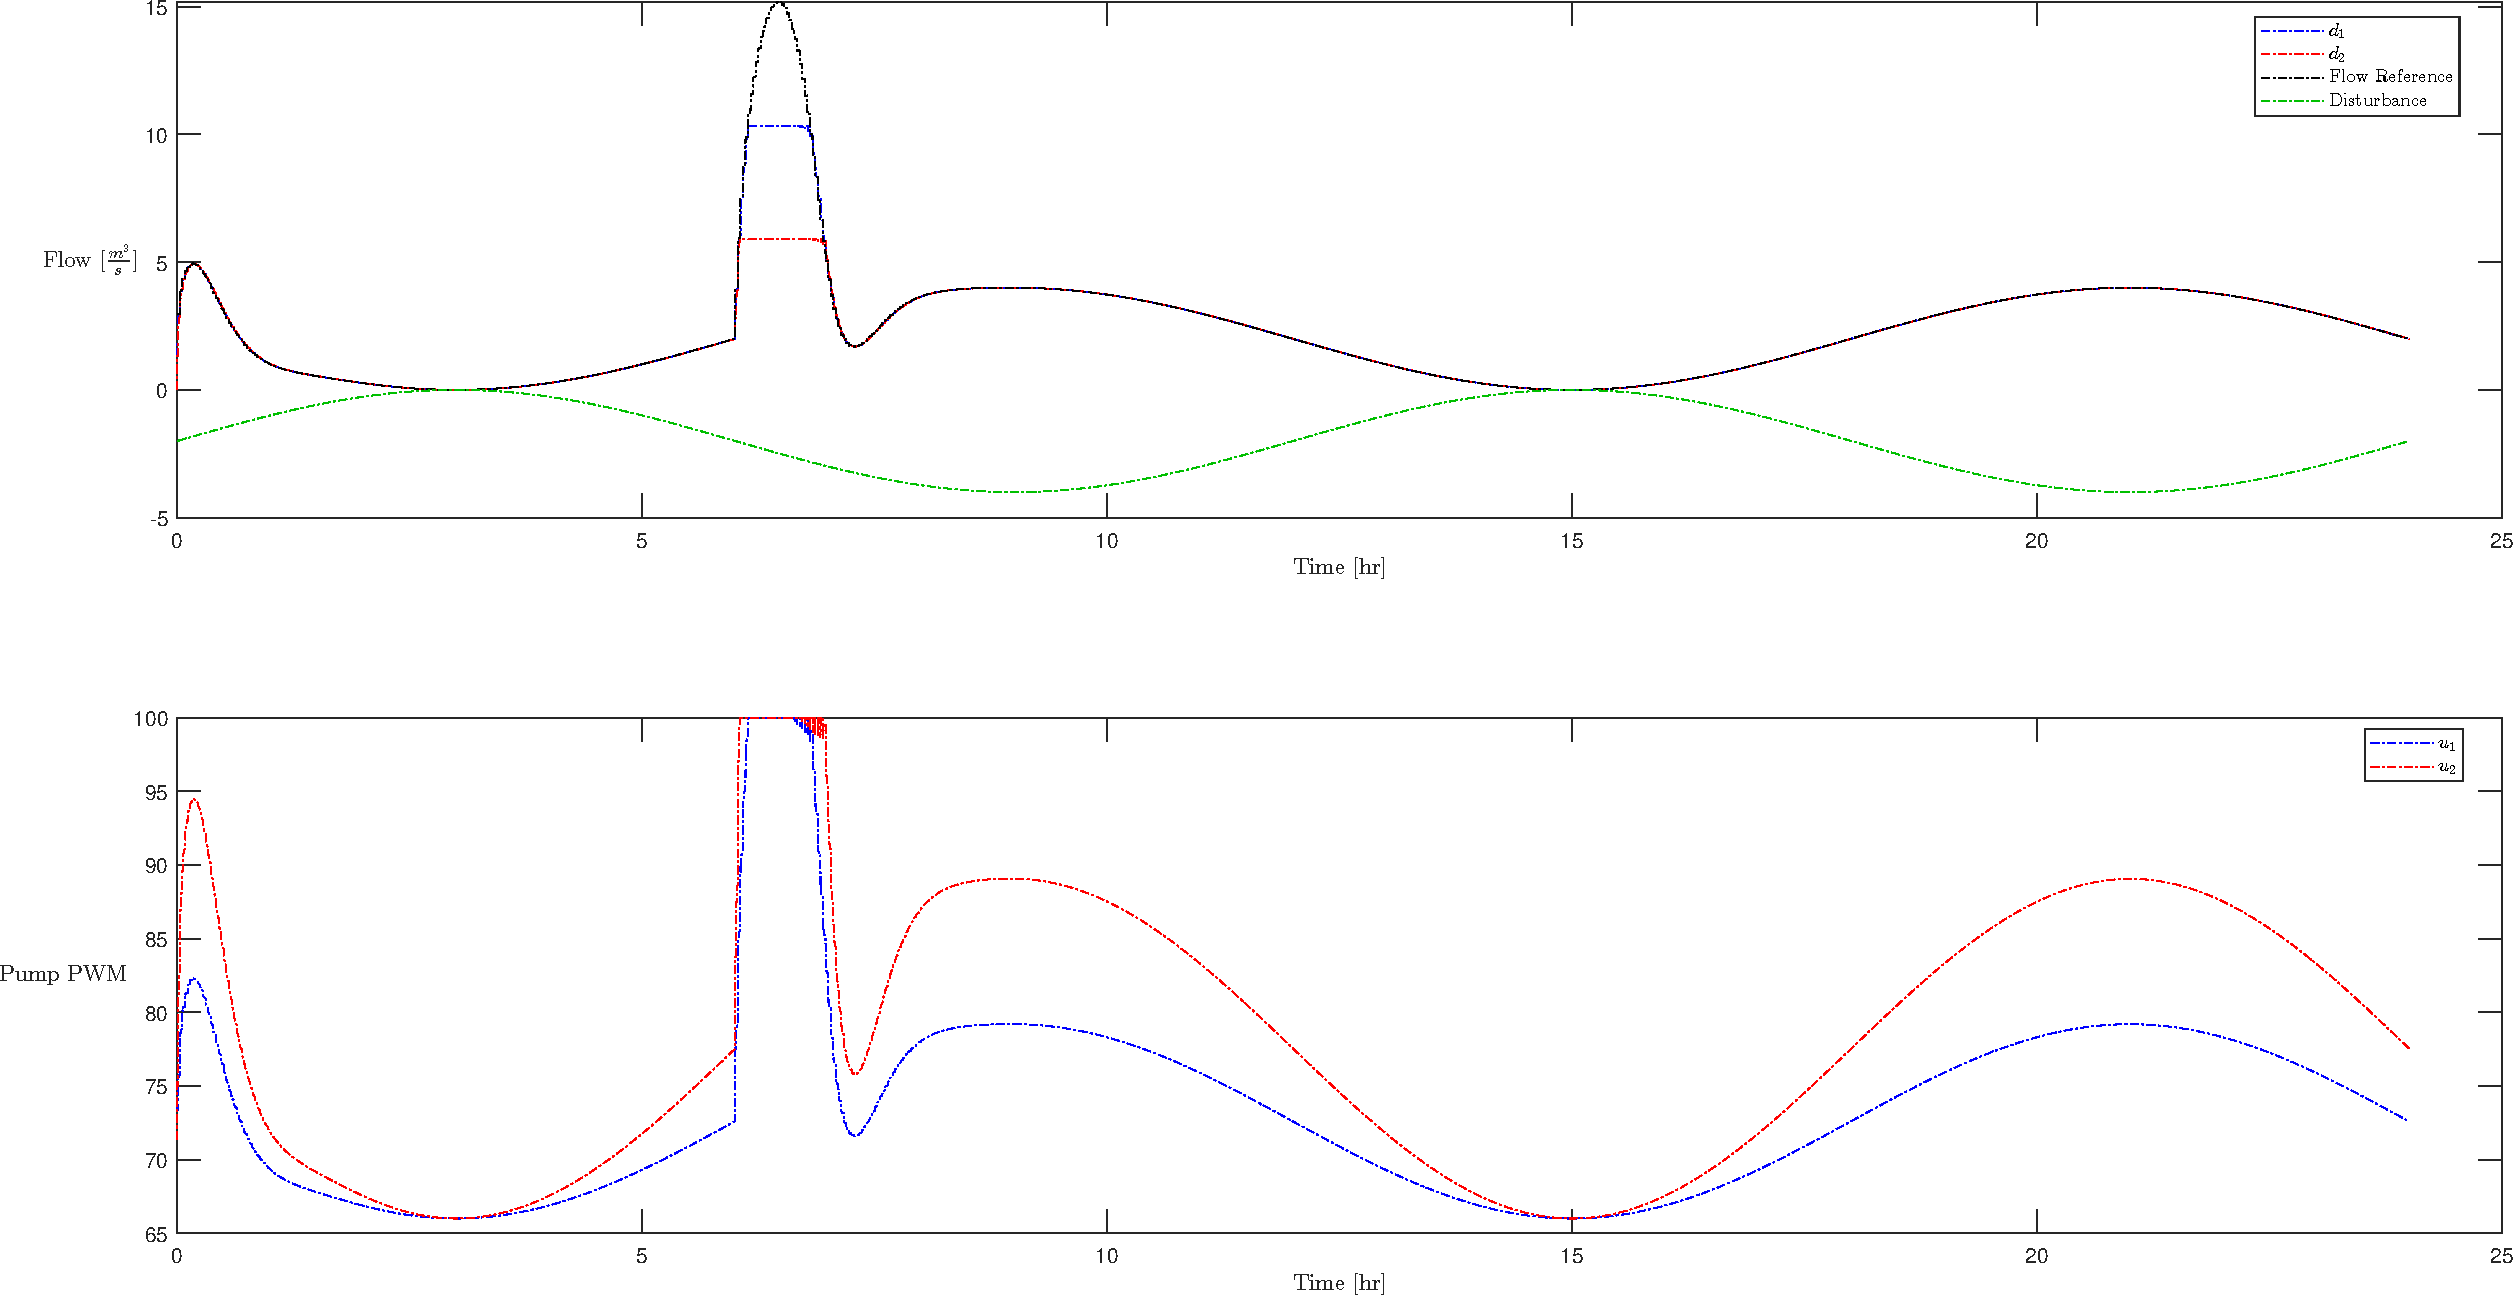
\includegraphics[height=4cm, width=\linewidth]{Graphics/FullSimFlows.pdf}
	\caption{Inner loop, cascaded simulation.}
	\label{fig:FullSimFlows}
\end{figure}

We note, as before, offset-free tracking. There is some overshoot after the reference change from $p_{ref} = 2 \ \si{bar}$ to $p_{ref} = 5 \ \si{bar}$; this is caused by the clamping of the the pumps to their maximum operating speed when the desired flow reference from the outer loop becomes too large, as the outer loop does not have anti-windup functionality. We note additionally that, as expected, the outer loop compensates for the time-varying disturbance by sign-reversed injection of the disturbance as a control signal.



